\documentclass{article}
\usepackage{algorithm2e}
\usepackage{graphicx}

\DeclareGraphicsExtensions{.png}

\title{Neural Networks: Assignment 1}
\author{Candidate Number: 18512}

\begin{document}
\maketitle

\begin{centering}
\subsubsection*{Abstract}
\end{centering}
\noindent This report will detail the implementation of a single layer perceptron for the purposes of binary classification and linear regression. \\
\indent The perceptron was implemented in Python. No Neural Network libraries or toolkits were used. Matplotlib and Numpy were used to produce graphs.
\vspace{4mm}

\section*{Part A: Classification}
\subsubsection*{Training Procedure}
In this part, sequential gradient descent was used, as it is somewhat simpler to implement, and for such simple cases, there is no benefit in terms of what we want to demonstrate, to using a more complicated implementation. Batch gradient descent will be used in part 2 of this assignment, however. \\
\indent The Perceptron Criterion error function is used, because unlike more naive error functions, Perceptron Criterion function yields a value proportional to the (sum of the) distance from the decision boundary. This is useful because any change in weights will correspond to a change in the value that the error function yields, which allows us to calculate the gradient of the error function, which in turn allows us to learn the optimum decision boundary via gradient descent. If a change in weights does not correspond to a change in error, we cannot determine whether the weight adjustment improved or worsened our learned function. \\
\indent The choice of learning rate for this part is not terribly important - it should be large enough that it does not cause the algorithm to do unnecessary extra iterations, and not be so great as to prevent convergence. 0.1 was found to be sufficient. \\

The training procedure for sequential gradient descent is as follows: \\

\begin{algorithm}[H]{\textbf{Procedure}: GradientDescentSequential} \\
    \KwIn{trainingData, weights, learningRate}
    \SetAlgoLined
    \Begin{
        \While{any element of trainingData is incorrectly classified} {
            \For{each instance in trainingData} {
                \If{instance is correctly classified} {
                    update weights in proportion to learningRate so instance is (closer to being) correctly classified
                }
            }
        }
    }
    \KwResult{weights}
\end{algorithm}
\vspace{4mm}

\noindent At the heart of this algorithm is the weight update step. To determine how we will update the weights, we use the Perceptron Criterion error function:
\[E^{Perc} = -\sum_{i = 1}^{m} \underline{x}_{i} . \underline{y}_{i} t_{i} \hspace{2mm} \textrm{for all misclassified} \hspace{2mm} x_{i}\]
With batch gradient descent, we can simply update every weight by the amount returned by this error function, multiplied by the learning rate. However, when applying this error function to sequential gradient descent, we get the following update rule:
\[w_{t+1} = w_{t} + \eta \underline{x}_{i} t_{i}\]
which is applied once for each instance over each epoch.
\subsection*{Question 1}
\indent For this question, initial weights were all zero as specified in the assignment brief.

\subsubsection*{Learnable Patterns}
The implemented single layer perceptron was able to learn four of the six given patterns:
\begin{center}
    \begin{tabular}{ l | c c c | l | c c c }
                & X1 & X2 & Label &         & X1 & X2 & Label \\
        \hline
        Pattern & 1  & 1  & +     & Pattern & 1  & 1  & -     \\
        Set 1   & 1  & 0  & -     & Set 2   & 1  & 0  & +     \\
                & 0  & 1  & +     &         & 0  & 1  & -     \\
                & 0  & 0  & -     &         & 0  & 0  & +     \\
        \hline
        Pattern & 1  & 1  & +     & Pattern & 1  & 1  & -     \\
        Set 3   & 1  & 0  & +     & Set 4   & 1  & 0  & -     \\
                & 0  & 1  & -     &         & 0  & 1  & +     \\
                & 0  & 0  & -     &         & 0  & 0  & +     \\
    \end{tabular}
\end{center}
Pattern sets 1 \& 2 are equivalent modulo the choice of class names, and as a result are learnt in the same number of iterations (2). The same is the case for pattern sets 3 \& 4. The ones that cannot be learnt are just so because they are not linearly separable i.e. there exists no linear boundary that separates all instances of one class from all instances of the other. These are given below:
\begin{center}
    \begin{tabular}{ l | c c c | l | c c c }
                & X1 & X2 & Label &         & X1 & X2 & Label \\
        \hline
        Pattern & 1  & 1  & +     & Pattern & 1  & 1  & -     \\
        Set 5   & 1  & 0  & -     & Set 6   & 1  & 0  & +     \\
                & 0  & 1  & -     &         & 0  & 1  & +     \\
                & 0  & 0  & +     &         & 0  & 0  & -     \\
    \end{tabular}
\end{center}
The following table shows the learned weights and number of iterations for each set of learnable patterns:
\begin{center}
    \begin{tabular}{ c | c | c | c | c }
        Pattern Set & Bias & Weight 1 & Weight 2 & Iterations \\
        \hline
        1           & 0    & -0.2     & 0        & 2          \\
        \hline
        2           & -0.1 & 0.2      & 0        & 2          \\
        \hline
        3           & 0    & 0        & -0.1     & 2          \\
        \hline
        4           & -0.1 & 0        & 0.1      & 2          \\
    \end{tabular}
\end{center}

The graphs below show the state of the decision boundary after each iteration, for pattern set 4: \\

\centerline{\textbf{Initial State}: Bias = 0, W1 = 0, W2 = 0}
\centerline{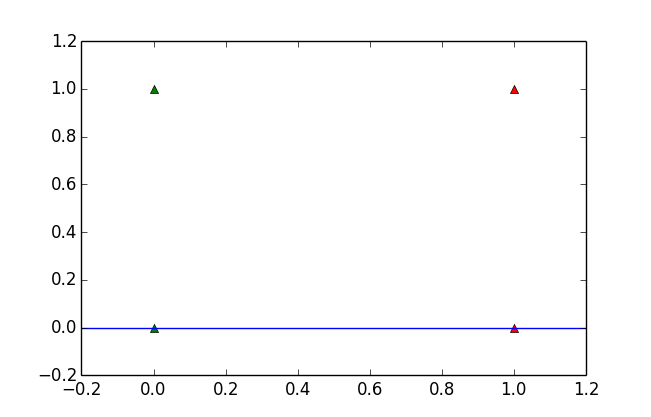
\includegraphics[width=200px]{partA1_iter1}}
\vspace{6mm}
\centerline{\textbf{After First Iteration}: Bias = 0, W1 = 0, W2 = 0.1}
\centerline{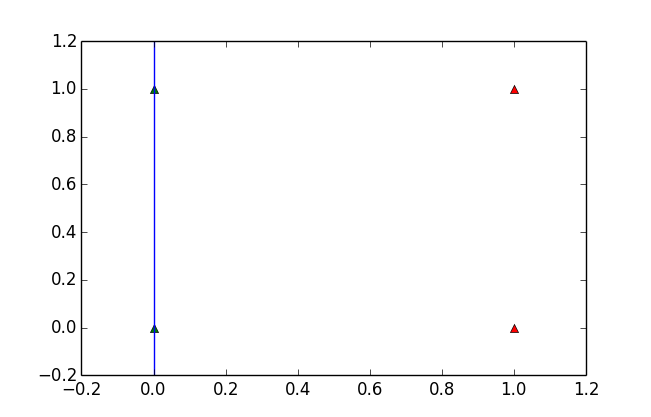
\includegraphics[width=200px]{partA1_iter2}}
\vspace{6mm}
\centerline{\textbf{After Second Iteration} (final state): Bias = -0.1, W1 = 0, W2 = 0.1}
\centerline{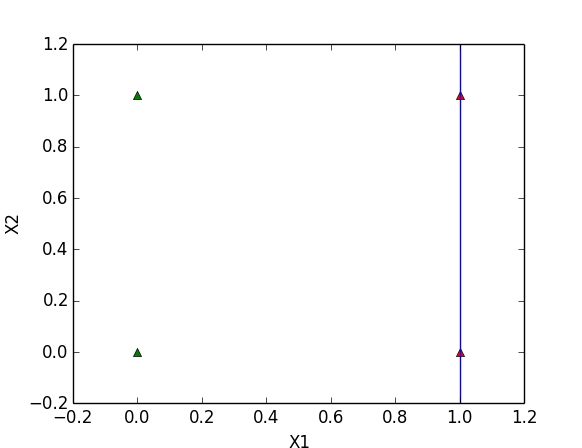
\includegraphics[width=200px]{partA1_iter3}}

\subsection*{Question 2}
In this question, the same code was used to learn the decision boundary as with question 1. The graph below shows the output of an example run of the implementation for this question: \\\\
\centerline{\textbf{Example Instances \& Decision Boundary}}
\centerline{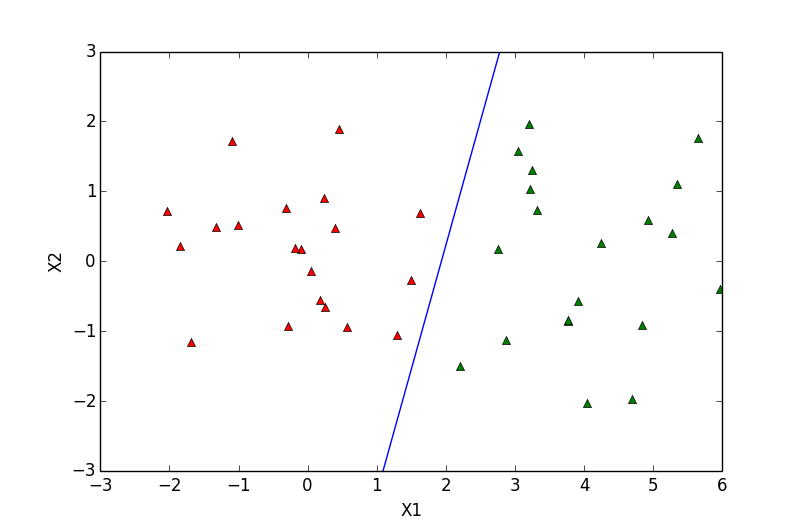
\includegraphics[width=400px]{partA2_1}}

\noindent The graph below shows the boundary learned for a non-linearly separable set of points - the decision boundary is not able to classify all points correctly, and, moreover, it is far from optimal, as we can see from the graph. It does not describe the data well. Since the algorithm used does not terminate for non-linearly separable data (it will never be the case that all points are correctly classified), an iteration limit must be imposed for non-linearly separable data. In the example below, the algorithm was limited to 100 iterations (over all data points i.e. 100 epochs). \\\\
\centerline{\textbf{Example of non-linearly separable Instances \& resulting Decision Boundary}}
\centerline{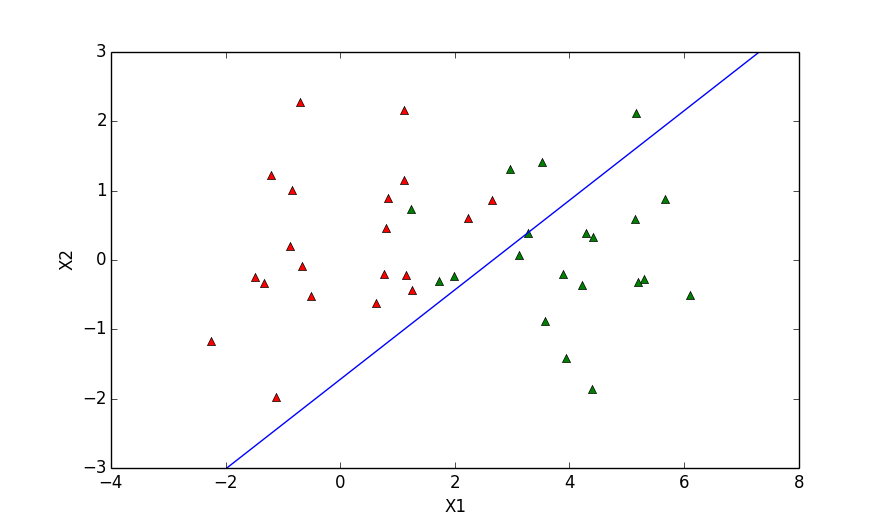
\includegraphics[width=400px]{partA2_2}}
\vspace{6mm}

\noindent The graphs below show how the decision boundary moves after each iteration for a set of points that were learned in 3 iterations: \\
\begin{center}
\textbf{Initial State}: Bias = 0, W1 = 0, W2 = 0 \\
\centerline{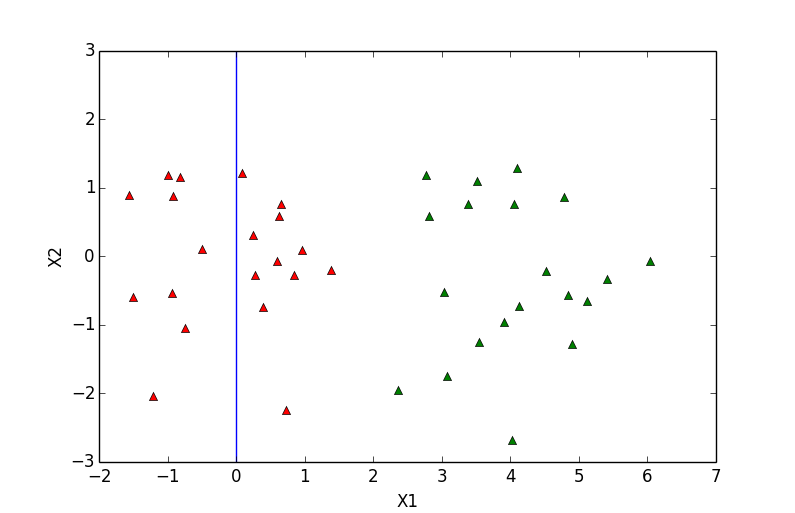
\includegraphics[width=400px, height=220px]{partA2_iter0}}
\vspace{2mm}
\rule{8cm}{0.4pt} \\
\vspace{2mm}
\textbf{After First Iteration}: Bias = 0.3, W1 = -0.22, W2 = 0.04 \\
\centerline{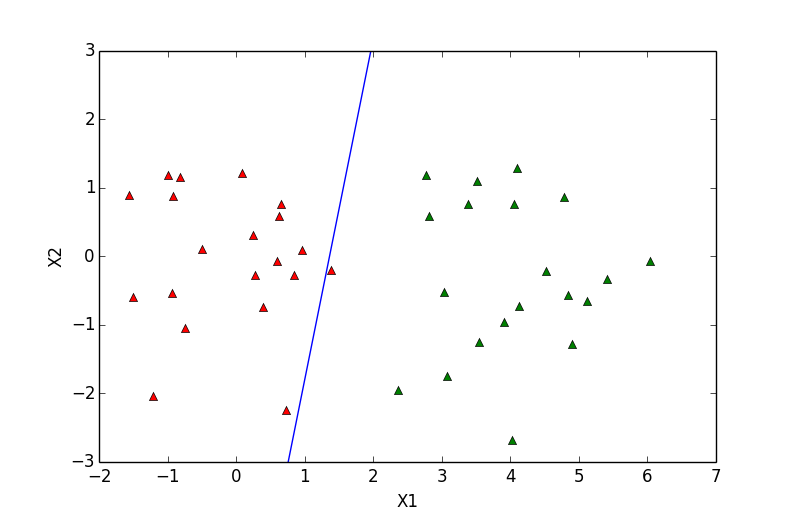
\includegraphics[width=400px, height=220px]{partA2_iter1}}
\vspace{2mm}
\rule{8cm}{0.4pt} \\
\vspace{2mm}
\textbf{After Second Iteration}: Bias = 0.4, W1 = -0.43, W2 = -0.05 \\
\centerline{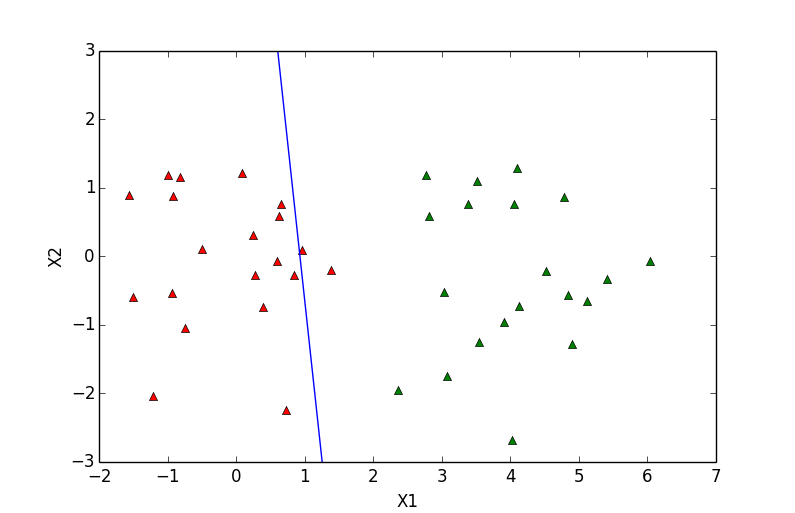
\includegraphics[width=400px, height=220px]{partA2_iter2}}
\vspace{2mm}
\rule{8cm}{0.4pt} \\
\vspace{2mm}
\textbf{After Third Iteration} (final state): Bias = 0.5, W1 = -0.33, W2 = -0.04 \\
\centerline{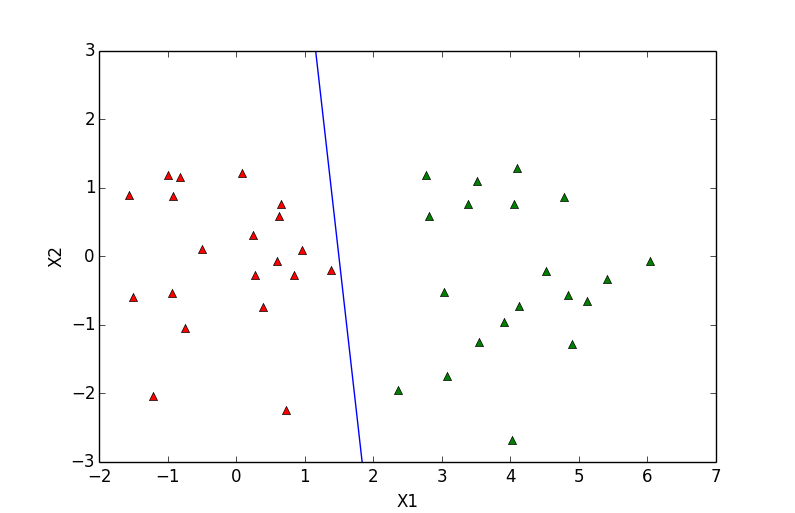
\includegraphics[width=400px, height=220px]{partA2_iter3}}
\vspace{2mm}
\rule{8cm}{0.4pt} \\
\vspace{2mm}
\end{center}

\noindent Given the function used to generate the data, the ideal decision boundary would be the vertical line X1 = 2. In all cases we have seen, the noise in the data prevents such a line from being learned. With a larger dataset, this noise would likely not affect the line to such a degree, however the larger the dataset becomes, the less likely it is that the dataset is linearly separable. \\
\indent Using a sigmoidal activation function provides an estimate of certainty for a classification decision. It was found not to help generalise (i.e. learn weights closer to the original function) for linearly separable input, because if an instance is correctly classified, we do not adjust the weights for it at all. With non-linearly separable data, however, generalisation is improved, as we consider the contribution of instances closer to the decision boundary to be less significant, while instances extremely far from it do not contribute significantly more to the movement of the decision boundary than those that exemplify data in a given class.

\section*{Part B: Regression}
For this part, batch gradient descent is used - this is because it makes it easier to determine when the algorithm should conclude. Determining when the algorithm should conclude is very simple with a classification task - we can simply stop iterating when all points are correctly classified. With regression, however, this will never be the case, since labels are continuous. Instead, we use a \emph{convergence threshold} - this is a value, which is determined before execution, that determines when the algorithm concludes. If an iteration takes place, and none of the weights change by an amount greater in magnitude than our convergence threshold, we consider the algorithm to have converged. \\
\indent The Perceptron Criterion error function is also used in this implementation, for the same reasons as with part A.
A much lower learning rate is required due to the nature of the training procedure - The large feature values for our instances cause divergence (i.e. the algorithm never converges and the weights go off to infinity) if we do not use a very small learning rate to compensate. \\
\indent The training procedure for this part of the assignment is given below:

\vspace{4mm}
\begin{algorithm}[H]{\textbf{Procedure}: GradientDescentBatch} \\
    \KwIn{trainingData, weights, learningRate}
    \SetAlgoLined
    \Begin{
        \While{algorithm not converged}{
            Calculate the average error across all trainingData, and adjust the weights appropriately, in proportion to learningRate
        }
    }
    \KwResult{weights}
\end{algorithm}
\vspace{4mm}
\subsection*{Question 1}

The tables below show weights learned by the network for different sets of points, each generated as specified, with 3 different ranges for random fluctuation. Interestingly, we can see that with small random fluctuations, we are able to learn a gradient that is relatively very close to the original function, but the learned bias deviates from the original function by a much greater degree. As the size of the random fluctuation increases, we can see that on average, the bias learned is much closer on average to the bias in the original function, although it fluctuates to a greater degree - the noise in the data is being learned as we add more noise into it. The learned gradient becomes further from the actual function as the size of the random fluctuations increase, again the random noise we introduce is being learned by the network, making generalisation worse.

\begin{center}
    \textbf{Fluctuations: -10 to +10}        \\
    \begin{tabular}{ r | l | l | l }
        \hline
        & Bias (3SF) & W1 (3SF) & Iterations \\
        \hline
        & 2.51       & 0.401    & 27368      \\
        & 0.141      & 0.408    & 2252       \\
        & 0.00388    & 0.422    & 20         \\
        & 0.897      & 0.416    & 12491      \\
        & 2.14       & 0.402    & 24536      \\
        & 1.78       & 0.406    & 21486      \\
        & 0.556      & 0.427    & 8258       \\
        & 2.48       & 0.406    & 27178      \\
        & 0.661      & 0.417    & 9623       \\
        & 2.28       & 0.399    & 25610      \\
        \hline
   Avg: & 1.34       & 0.410    & 15882.2    \\
        \hline
    \end{tabular}
\end{center}
\vspace{5mm}
\begin{center}
    \textbf{Fluctuations: -30 to +30}        \\
    \begin{tabular}{ r | l | l | l }
        \hline
        & Bias (3SF) & W1 (3SF) & Iterations \\
        \hline
        & 3.41       & 0.363    & 29741      \\
        & 0.795      & 0.414    & 11289      \\
        & 0.00367    & 0.438    & 20         \\
        & 1.62       & 0.394    & 19988      \\
        & 5.60       & 0.403    & 30259      \\
        & 0.00306    & 0.413    & 20         \\
        & 0.00320    & 0.415    & 20         \\
        & 2.79       & 0.425    & 29439      \\
        & 1.63       & 0.410    & 20108      \\
        & 0.603      & 0.423    & 8879       \\
        \hline
   Avg: & 1.65       & 0.410    & 14976.3    \\
        \hline
    \end{tabular}
\end{center}
\vspace{5mm}
\begin{center}
    \textbf{Fluctuations: -50 to +50}        \\
    \begin{tabular}{ r | l | l | l }
        \hline
        & Bias (3SF) & W1 (3SF) & Iterations \\
        \hline
        & 11.4       & 0.356    & 63914      \\
        & 0.00390    & 0.427    & 20         \\
        & -2.93      & 0.471    & 30432      \\
        & -0.297     & 0.445    & 4733       \\
        & -2.17      & 0.460    & 24792      \\
        & 7.90       & 0.382    & 53755      \\
        & 1.13       & 0.382    & 15103      \\
        & 0.0235     & 0.43     & 342        \\
        & 9.42       & 0.330    & 58534      \\
        & 4.41       & 0.367    & 39177      \\
        \hline
   Avg: & 2.89       & 0.405    & 29080.2    \\
        \hline
    \end{tabular}
\end{center}

\noindent The convergence threshold used was 0.000059, which was chosen because it is small enough that we do not conclude early because of our low learning rate - since our learning rate has to be very small for the algorithm to converge, the weights change by very small amounts each iteration. We need a convergence threshold that allows the weights to change very slowly without 'cutting short' the iteration because changes in the weights are very small. \\
\indent The learning rate used was 0.00000012, which is small enough that the algorithm will converge and not diverge, but not so small as to necessitate many additional iterations such that the algorithm concludes in an unreasonably long amount of time. \\
\indent The graph below shows some example output with fluctuations of -10 to +10.
\begin{center}
\textbf{Example output for part B1}\\
\centerline{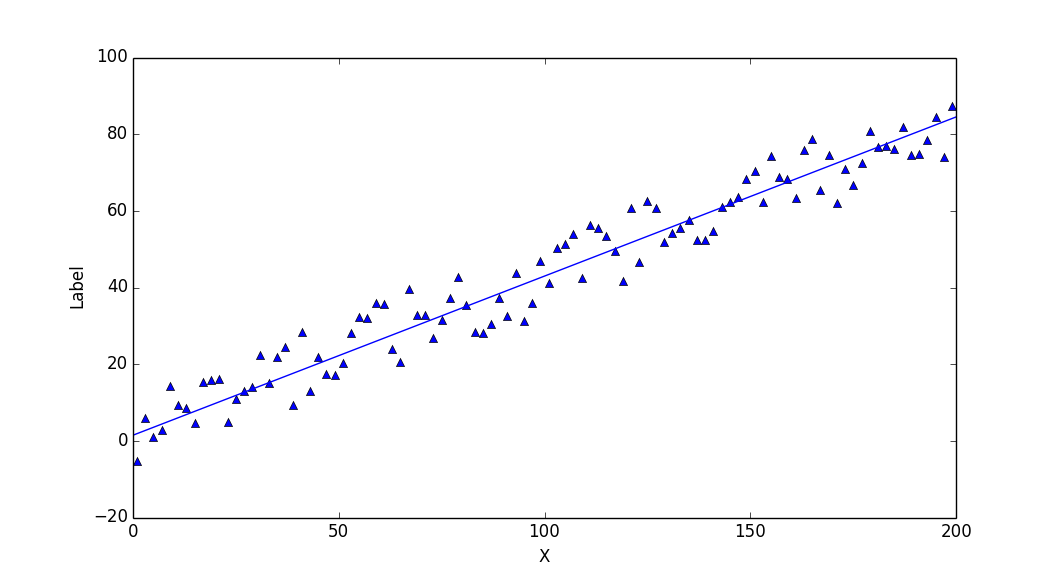
\includegraphics[width=400px, height=220px]{partB1}}
\vspace{2mm}
\end{center}

\subsection*{Question 2}
For this task, again, the learning rate and convergence threshold had to be very small to allow convergence without causing early termination. The used learning rate was 0.00000012 and the convergence threshold was 0.00003. \\
\indent Since two feature values are used, we can plot the values as points in 3D space, and the learned regressor is a plane in this 3D space. The graphs below show an example output plane of regression, for the same set of points \& weights, viewed from different angles.

\begin{center}
\centerline{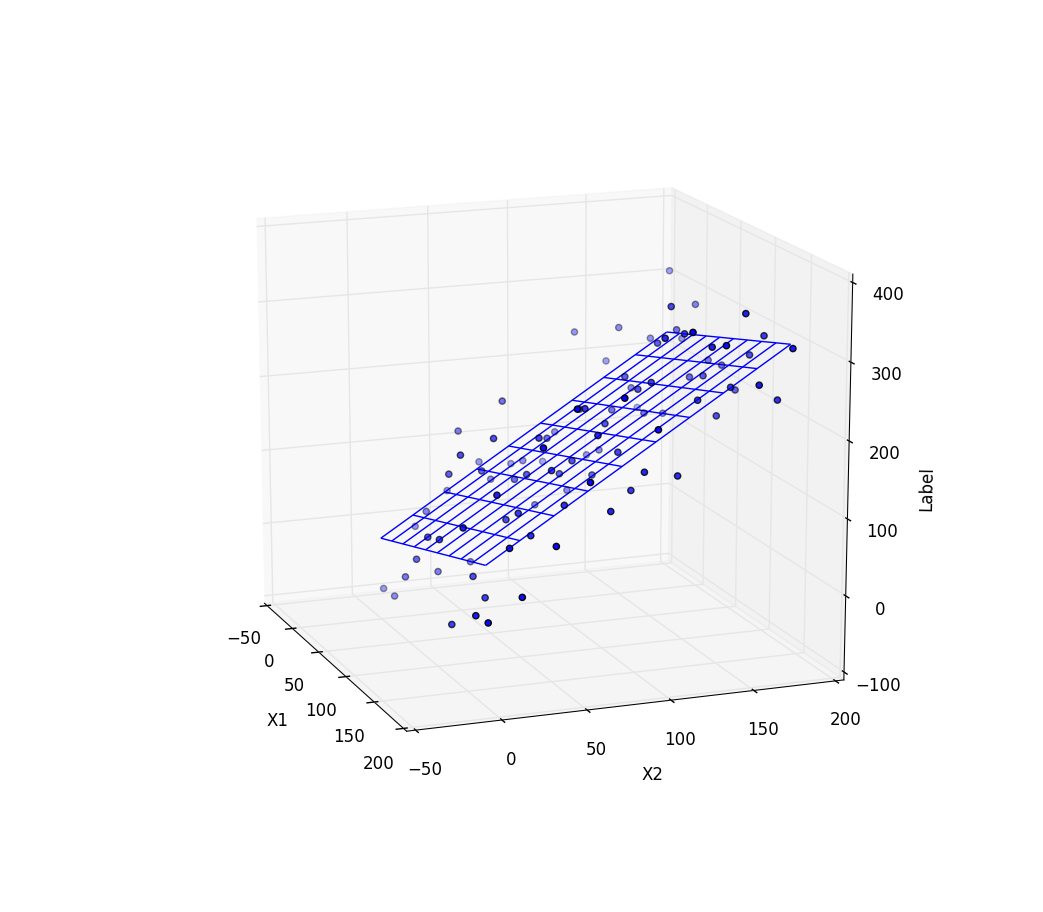
\includegraphics[width=400px, height=400px]{partB2_1}}
\vspace{2mm}
\centerline{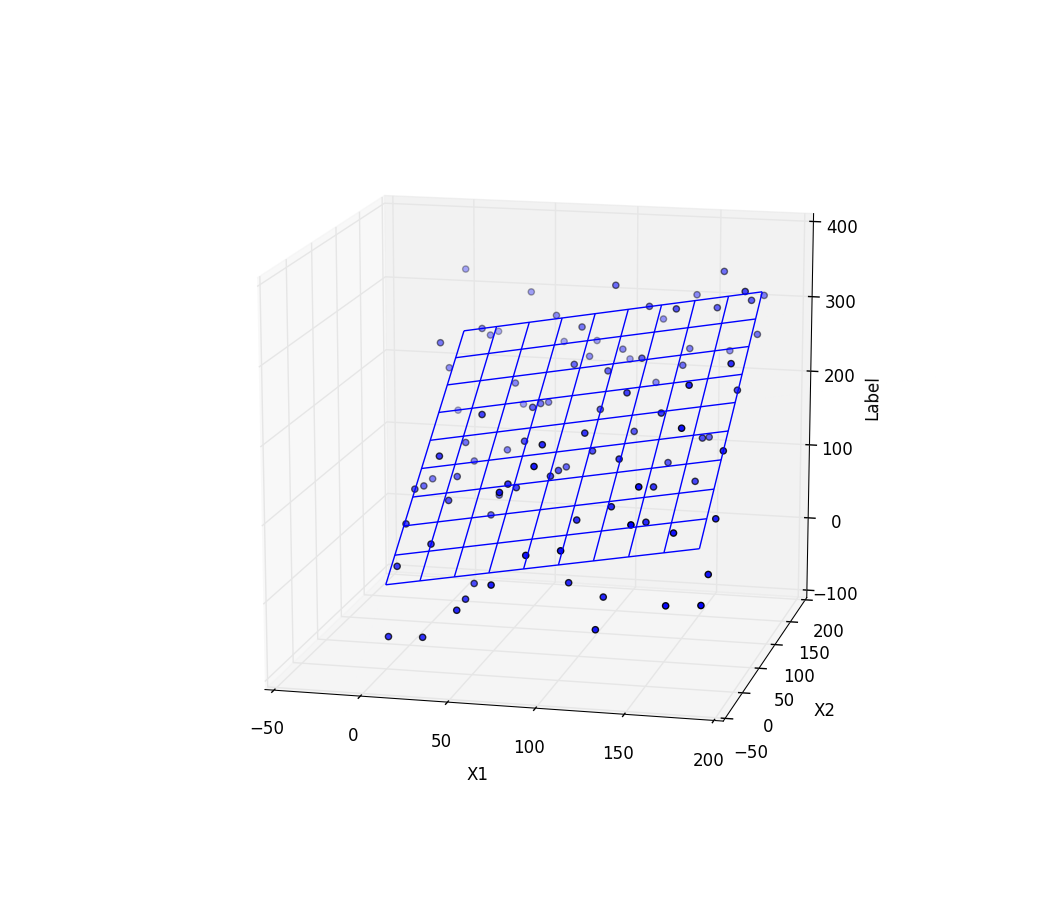
\includegraphics[width=400px, height=400px]{partB2_2}}
\vspace{2mm}
\centerline{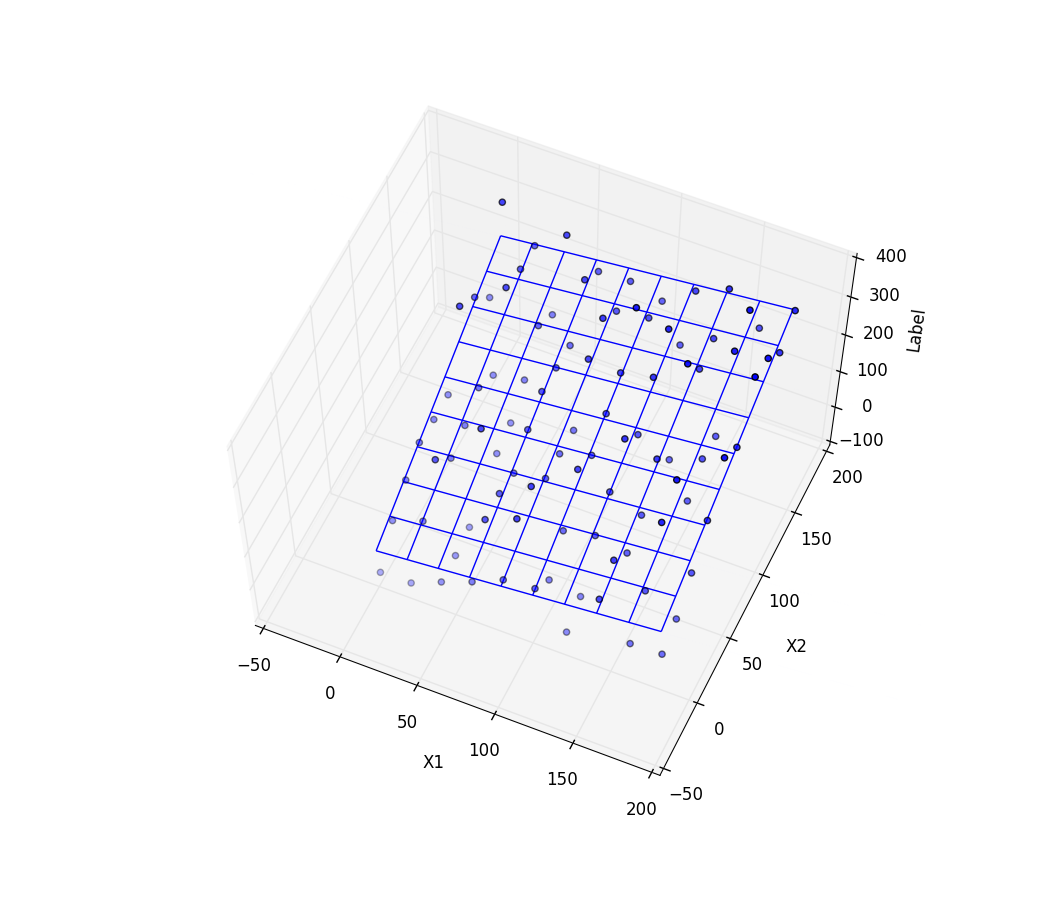
\includegraphics[width=400px, height=400px]{partB2_3}}
\vspace{2mm}
\textbf{Bias: 0.00478, W1: 0.397, W2: 1.35 (3SF)}\\
\end{center}

\noindent We can see from the weight \& bias values above, that the network produces weight values that are relatively even closer to those used in the original function, compared with those in part B1. \\
\indent Again the random fluctuations were adjusted as specified in the tables below, which show sample weights for runs of the algorithm on different sets of random data. In this case, however, the average predicted bias does not get closer to the original bias as the random fluctuation size increases, as it did with part B1. For all weights and the bias, the values are further from that of the original function - again, noise introduced into data is being learned.

\begin{center}
    \textbf{Fluctuations: -100 to +100}        \\
    \begin{tabular}{ r | l | l | l | l }
        \hline
        & Bias (3SF) & W1 (3SF) & W2 (3SF) & Iterations \\
        \hline
 & 0.00995& 0.437& 1.33& 10363 \\
 & 0.00818& 0.466& 1.35& 10330 \\
 & 0.0121& 0.350& 1.45& 10874 \\
 & 0.00860& 0.229& 1.41& 11051 \\
 & 0.00996& 0.371& 1.38& 10657 \\
 & 0.00214& 0.438& 1.32& 10318 \\
 & 0.00717& 0.288& 1.59& 11290 \\
 & 0.00584& 0.455& 1.31& 10243 \\
 & 0.00662& 0.375& 1.51& 10933 \\
 & 0.0114& 0.355& 1.53& 11020 \\
        \hline
Avg: & 0.00820& 0.376& 1.424& 10707.9 \\
        \hline
    \end{tabular}
\end{center}

\begin{center}
    \textbf{Fluctuations: -200 to +200}        \\
    \begin{tabular}{ r | l | l | l | l }
        \hline
        & Bias (3SF) & W1 (3SF) & W2 (3SF) & Iterations \\
        \hline
& 0.00336& 0.209& 1.52& 11311 \\
& 0.00884& 0.314& 1.29& 10575 \\
& 0.0101& 0.228& 1.32& 10842 \\
& 0.00125& 0.437& 1.23& 10056 \\
& 0.00590& 0.484& 1.52& 10728 \\
& 0.0108& 0.459& 1.24& 10027 \\
& 0.00571& 0.430& 1.30& 10279 \\
& 0.00875& 0.503& 1.16& 9602 \\
& 0.00352& 0.534& 1.08& 9123 \\
& 0.0130& 0.551& 1.26& 9798 \\
        \hline
        Avg: & 0.00713& 0.415& 1.29& 10234.1\\
        \hline
    \end{tabular}
\end{center}

\begin{center}
    \textbf{Fluctuations: -300 to +300}        \\
    \begin{tabular}{ r | l | l | l | l }
        \hline
        & Bias (3SF) & W1 (3SF) & W2 (3SF) & Iterations \\
        \hline
& 0.00676& 0.446& 1.13& 9683 \\
& 0.0190& 0.286& 1.53& 11176 \\
& -0.00442& 0.419& 1.64& 11132 \\
& 0.0104& 0.188& 1.54& 11372 \\
& 0.0232& 0.385& 1.43& 10749 \\
& 0.00381& 0.449& 1.54& 10855 \\
& 0.00310& 0.507& 1.34& 10186 \\
& -0.0187& -0.0135& 1.80& 12117 \\
& 0.0199& 0.429& 1.38& 10512 \\
& 0.00244& 0.413& 1.49& 10817 \\
        \hline
        Avg: & 0.00657& 0.351& 1.48&10864.4\\
        \hline
    \end{tabular}
\end{center}

\section*{Appendix}
Source code is supplied in the submitted archive in the file assignment1.py. To run, python 2.7, numpy \& matplotlib are required.

\subsection*{Source code}

\begin{verbatim}

#!/bin/python2
# Candidate No: 18512
import random, math
import matplotlib.pyplot as plot
from mpl_toolkits.mplot3d import Axes3D
import numpy as np

POSITIVE = 1
NEGATIVE = -1

class Instance:
    '''
    An Instance contains:
        data  - a list of values for each dimension
        label - the class label
    '''
    def __init__(self, data, label):
        self.data  = data
        self.label = label

    def __str__(self):
        '''
        Get a nice string representation of this Instance object
        '''
        return ''.join(['DATA: ', str(self.data), ', LABEL: ', str(self.label)])

class Weights:

    def __init__(self, bias, weights):
        self.bias    = bias
        self.weights = weights

    def copy(self):
        return Weights(self.bias, [w for w in self.weights])

    def __str__(self):
        '''
        Get a nice string representation of this Weights object
        '''
        return ''.join(['BIAS: ', str(self.bias), ', WEIGHTS: ',
                str(self.weights)])

def grad_desc_sequential(training_instances, wts
        , learning_rate = 0.1
        , iteration_cap = 100
        , collect_weights = False
        ):
    '''
    Learn a perceptron from the given training instances. If the default weights
    are used, then the given instances must be 2-dimensional. The algorithm used
    is sequential gradient descent.
        If collect_weights is set, the weights will be recorded at each epoch
    and returned in a list, rather than just returning the final weights.
    '''

    if collect_weights:
        weights_list = []

    converged = False
    iterations = 0
    while not converged and iterations < iteration_cap:

        if collect_weights: weights_list.append(wts.copy())

        converged = True
        iterations = iterations + 1

        for inst in training_instances:
            if heaviside_classify(wts, inst) != inst.label:
                converged = False
                for i in range(len(wts.weights)):
                    wts.weights[i] = wts.weights[i] + (
                            learning_rate * inst.data[i] * inst.label)
                wts.bias = wts.bias + (learning_rate * inst.label)

    return (weights_list if collect_weights else wts, iterations)

def grad_desc_batch(training_instances, wts
        , learning_rate = 0.1
        , iteration_cap = 100
        , convergence_threshold = 0.1
        ):
    iterations = 0
    num_insts = len(training_instances)

    while iterations < iteration_cap:

        iterations = iterations + 1

        new_wts = wts.copy()

        # Adjust the bias
        new_wts.bias = wts.bias - (learning_rate * ( \
                sum([activation(wts, inst) - inst.label \
                for inst in training_instances])/num_insts))
        
        # Adjust the weight for each dimension
        for i in range(len(wts.weights)):
            new_wts.weights[i] = wts.weights[i] - (learning_rate * ( \
                    sum([(activation(wts, inst) - inst.label) * inst.data[i] \
                    for inst in training_instances])/num_insts))


        # Conclude if the weights have converged
        if converged(wts, new_wts, convergence_threshold): break

        wts = new_wts

    return new_wts, iterations

def converged(wts1, wts2, threshold):
    '''
    Compare two weight sets to see if a weight updating algorithm has converged.
    The threshold represents an allowed degree of deviation in the given weights
    such that convergence is still indicated
    '''
    if len(wts1.weights) != len(wts2.weights):
        raise Exception(
                'Mismatched dimensions for weights & instance in converged()')
    diffs = [abs(wts1.weights[i] - wts2.weights[i]) \
            for i in range(len(wts1.weights))]
    diffs.append(abs(wts1.bias - wts2.bias))
    return max(diffs) < threshold

def heaviside_classify(wts, inst):
    '''
    Get the class of an instance from the supplied weights using a heaviside
    function
    '''
    return POSITIVE if activation(wts, inst) >= 0 else NEGATIVE

def sigmoid_classify(wts, inst, coefficient=1):
    '''
    Derive a value that represents both a class (+1 for values greater than 0,
    -1 for values less than 0) and a degree of certainty for our class decision.
    The more extreme the value, the more certain our decision is. The closer to
    0 the value is, the less certain we are.
        A sigmoidal function S(t) = 1 / 1 - e^-ax, where a is the (optionally)
    given coefficient, and x is the dot product of the given weight & instance,
    is used.
    '''
    return 1 / (1 + (math.e ** (-1 * coefficient * activation(wts, inst))))

def tanh_classify(wts, inst):
    '''
    This function uses the hyperbolic tangent function to obtain a degree of
    certainty for classification, as with sigmoid_classify
    '''
    return math.tanh(activation(wts, inst))


def activation(wts, inst):
    '''
    The activation function for a perceptron - the dot product of the weights
    with the instance's features, plus the bias (although the bias can be seen
    as the weight on a feature that always has value 1)
    '''
    return dot(wts.weights, inst.data) + wts.bias

def dot(x, y):
    '''
    Compute the dot product of two vectors
    '''
    if len(x) is not len(y):
        raise Exception('Mismatched dimensions for weights & instance in dot()')

    return sum(map(lambda xi, yi: xi * yi, x, y))

def doPartA1():
    instance_sets = [
        [ Instance([0, 0], POSITIVE), Instance([1, 0], POSITIVE)
        , Instance([0, 1], NEGATIVE), Instance([1, 1], NEGATIVE)
        ],
        [ Instance([0, 0], POSITIVE), Instance([1, 0], NEGATIVE)
        , Instance([0, 1], POSITIVE), Instance([1, 1], NEGATIVE)
        ],
        [ Instance([0, 0], POSITIVE), Instance([1, 0], NEGATIVE)
        , Instance([0, 1], NEGATIVE), Instance([1, 1], POSITIVE)
        ],
        [ Instance([0, 0], NEGATIVE), Instance([1, 0], NEGATIVE)
        , Instance([0, 1], POSITIVE), Instance([1, 1], POSITIVE)
        ],
        [ Instance([0, 0], NEGATIVE), Instance([1, 0], POSITIVE)
        , Instance([0, 1], NEGATIVE), Instance([1, 1], POSITIVE)
        ],
        [ Instance([0, 0], NEGATIVE), Instance([1, 0], POSITIVE)
        , Instance([0, 1], POSITIVE), Instance([1, 1], NEGATIVE)
        ]]

    print '--- SEQUENTIAL ---'
    for insts in instance_sets:
        seq_wts, seq_iters = grad_desc_sequential(insts,
                Weights(0.0, [0.0, 0.0]))
        for i in insts:
            print 'INST:', i.data, 'LABEL:', i.label, 'CLASS:', \
                    str(heaviside_classify(seq_wts, i))
        print seq_wts, '\n', 'ITERATIONS: ', seq_iters, '\n'

    print '--- BATCH ---'
    for insts in instance_sets:
        bat_wts, bat_iters = grad_desc_batch(insts, Weights(0.0, [0.0, 0.0]),
                convergence_threshold=0.01)
        for i in insts:
            print 'INST:', i.data, 'LABEL:', i.label, 'CLASS:', \
                    str(heaviside_classify(bat_wts, i))
        print bat_wts, '\n', 'ITERATIONS: ', bat_iters, '\n'

    # Illustrate procedure with instance_sets[4] using sequential by showing the
    # graph after each iteration
    wts_list, iters = grad_desc_sequential(instance_sets[3],
            Weights(0.0, [0.0, 0.0]), collect_weights=True)
    negX1vals = [i.data[0] for i in instance_sets[3] if i.label is NEGATIVE]
    negX2vals = [i.data[1] for i in instance_sets[3] if i.label is NEGATIVE]
    posX1vals = [i.data[0] for i in instance_sets[3] if i.label is POSITIVE]
    posX2vals = [i.data[1] for i in instance_sets[3] if i.label is POSITIVE]
    iter_num = 0
    for wts in wts_list:
        iter_num = iter_num + 1
        print 'ITERATION', iter_num, 'OF', iters, ':', wts
        # Generate two points on the decision boundary that we can use to draw
        # the line
        linex1s = [-0.2, 1.2]
        linex2s = [-1 * (wts.bias + (x1 * wts.weights[1]))/(wts.weights[0] \
                if wts.weights[0] != 0 else 0.000000001) for x1 in linex1s]

        # Plot the points & line
        plot.plot(posX2vals, posX1vals, 'r^', negX2vals, negX1vals, 'g^',
                linex1s, linex2s, linewidth=1.0)
        plot.xlabel('X1')
        plot.ylabel('X2')
        plot.ylim([-0.2, 1.2])
        plot.xlim([-0.2, 1.2])
        plot.show()

def doPartA2():
    # Generate random data as specified:
    posX1vals = [random.gauss(0, 1) for x in range(20)]
    posX2vals = [random.gauss(0, 1) for x in range(20)]
    negX1vals = [random.gauss(4, 1) for x in range(20)]
    negX2vals = [random.gauss(0, 1) for x in range(20)]
    insts = []
    for i in range(20):
        insts.append(Instance([posX1vals[i], posX2vals[i]], POSITIVE))
        insts.append(Instance([negX1vals[i], negX2vals[i]], NEGATIVE))

    # Train the perceptron
    wts, iterations = grad_desc_sequential(insts, Weights(0.0, [0.0, 0.0]))

    # Generate two points on the decision boundary that we can use to draw the
    # line
    linex2s = [3.0, -3.0]
    linex1s = [-1 * (wts.bias + (x2 * wts.weights[1]))/wts.weights[0]
            for x2 in linex2s]

    print 'Decision boundary learnt in', iterations, 'iterations'

    # Plot the points & line
    plot.plot(posX1vals, posX2vals, 'r^', negX1vals, negX2vals, 'g^',
            linex1s, linex2s, linewidth=1.0)
    plot.xlabel('X1')
    plot.ylabel('X2')
    plot.show()
    """
    # Illustrate procedure with instance_sets[4] using sequential by showing the
    # graph after each iteration
    wts_list, iters = grad_desc_sequential(insts,
            Weights(0.0, [0.0, 0.0]), collect_weights=True)
    iter_num = 0
    for wts in wts_list:
        iter_num = iter_num + 1
        print 'ITERATION', iter_num, 'OF', iters, ':', wts
        # Generate two points on the decision boundary that we can use to draw
        # the line. Prevent division by zero by substituting zero values with a
        # very small number, that produces the same line.
        linex2s = [3.0, -3.0]
        linex1s = [-1 * (wts.bias + (x2 * wts.weights[1]))/(wts.weights[0]
                if wts.weights[0] != 0 else 0.000000001) for x2 in linex2s]

        # Plot the points & line
        plot.plot(posX1vals, posX2vals, 'r^', negX1vals, negX2vals, 'g^',
                linex1s, linex2s, linewidth=1.0)
        plot.xlabel('X1')
        plot.ylabel('X2')
        plot.show()
    """

def doPartB1():
    '''
    For this regression task, we think of our data as 1-dimensional, and the
    second dimension is essentially our class label.
    '''
    # y = 0.4*x + 3 + delta, delta = uniform random from -10 to +10
    data = [[x, (0.4 * x) + 3 + random.uniform(-10.0, 10.0)]
            for x in range(1, 200, 2)]
    insts = [Instance([d[0]], d[1]) for d in data]
    wts, iters = grad_desc_batch(insts
            , wts=Weights(0.0, [0.0])
            , learning_rate = 0.00012
            , iteration_cap = 70000
            , convergence_threshold = 0.000059
            )
    print wts, ', ITERS:', iters

    # Derive 2 points that lie on our learned regressorso that we can plot the
    # line
    linex1s = [0, 200]
    linex2s = [activation(wts, Instance([x1], None)) for x1 in linex1s]
    plot.plot([d[0] for d in data], [d[1] for d in data], 'b^',
            linex1s, linex2s, linewidth=1.0)
    plot.xlabel('X')
    plot.ylabel('Label')
    plot.show()

def doPartB2():
    # y = 0.4*x1 + 1.4*x2 + delta, delta = uniform random from -100 to +100
    data = [[x1, x2, (0.4 * x1) + (1.4 * x2) + random.uniform(-100, 100)]
            for x1 in range (1, 200, 20) for x2 in range(1, 200, 20)]
    insts = [Instance([d[0], d[1]], d[2]) for d in data]

    wts, iters = grad_desc_batch(insts
            , wts=Weights(0.0, [0.0, 0.0])
            , learning_rate = 0.00000012
            , iteration_cap = 30000
            , convergence_threshold = 0.000003
            )
    print wts, 'ITERS:', iters

    # Derive some points that lie on our regressor plane, such that we can draw
    # the plane nicely
    planeX1s = range(0, 200, 20)
    planeX2s = range(0, 200, 20)
    planeX1s, planeX2s = np.meshgrid(planeX1s, planeX2s)
    planeYs = [activation(wts, Instance([planeX1s[i], planeX2s[i]], None))
            for i in range(len(planeX1s))]
    fig = plot.figure()
    axis = fig.add_subplot(111, projection='3d')
    axis.scatter([i.data[0] for i in insts], [i.data[1] for i in insts],
            [i.label for i in insts])
    axis.plot_wireframe(planeX1s, planeX2s, planeYs)
    axis.set_xlabel('X1')
    axis.set_ylabel('X2')
    axis.set_zlabel('Label')
    plot.show()

if __name__ == "__main__":
    # Uncomment as required
    #doPartA1()
    doPartA2()
    #doPartB1()
    #doPartB2()
\end{verbatim}
\end{document}
